\justifying
\begin{problem}{\label{task_51}}
	Два грузи з масами $m_1$ та $m_2$ зв'язані легкою ниткою, перекинутою через нерухомий блок. Груз маси $m_1$ відпускають без поштовха. З яким прискоренням $a$ відносно стола рухаються грузи, якщо кеофіцієнт тертя другого груза об стіл рівен $\mu$? Яка сила натягу $T$? Як зміниться відповідь, якщо система буде знаходитись в ліфті, який рухається з прискоренням $a_0$ напрямленим вгору? (рис. \ref{fig:day51})
	\begin{figure}[h!]
		\centering
		\begin{subfigure}{.4\textwidth}
			\centering
			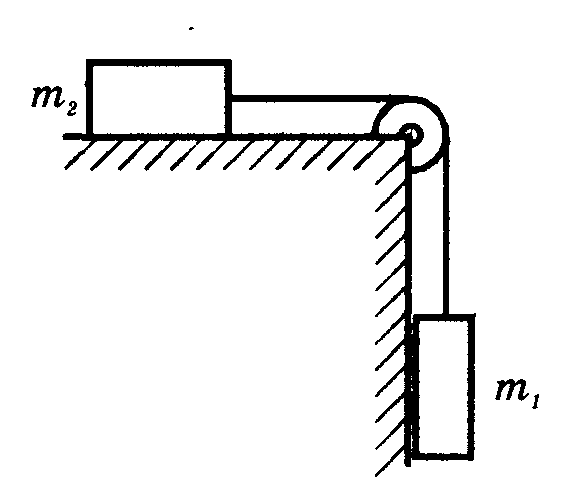
\includegraphics[width= 0.5\linewidth]{class5/day5_1}
			\caption{До задачі 5.1}
			\label{fig:day51}
		\end{subfigure}
		\begin{subfigure}{.4\textwidth}
			\centering
			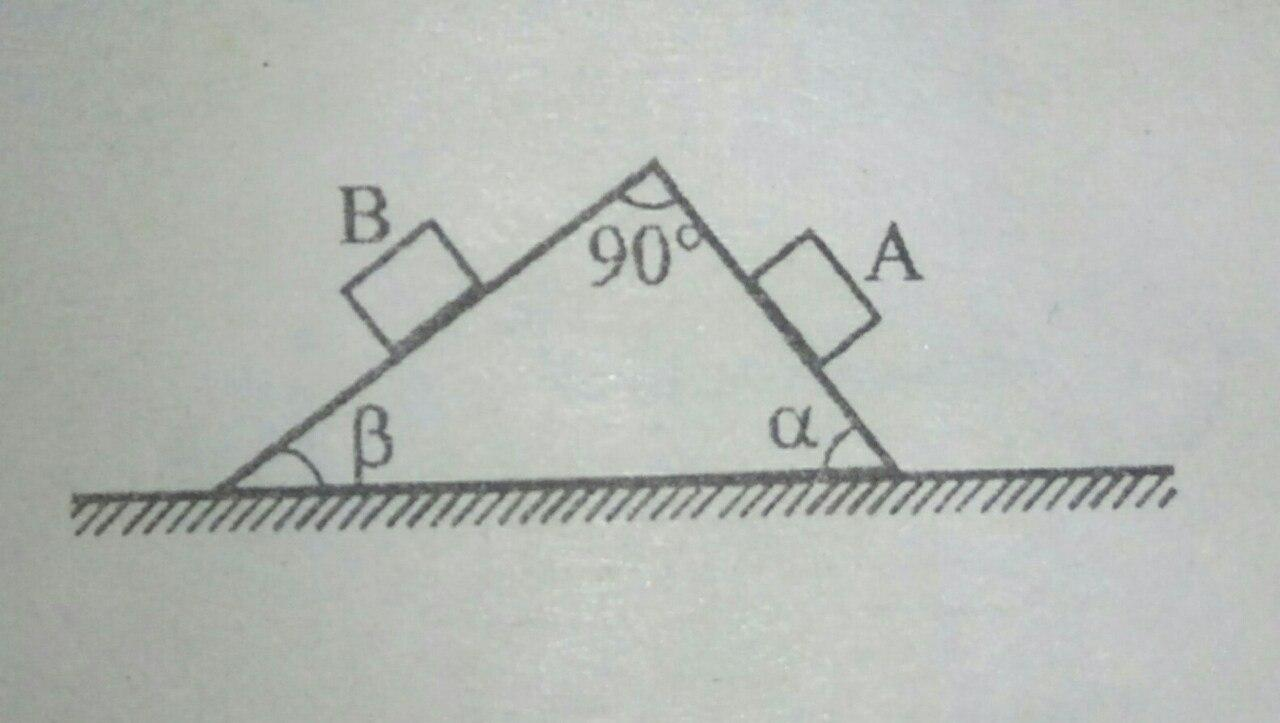
\includegraphics[width=0.5\linewidth]{class5/day5_02}
			\caption{До задачі 5.3}
			\label{fig:day502}
		\end{subfigure}
		\begin{subfigure}{.4\textwidth}
			\centering
			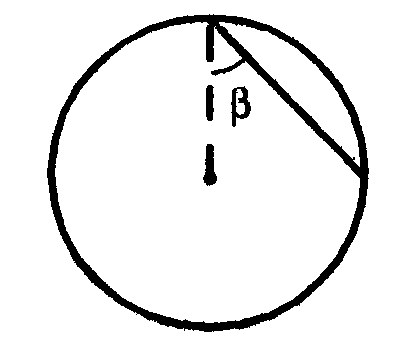
\includegraphics[width=0.5\linewidth]{class5/day5_3}
			\caption{До задачі 5.4}
			\label{fig:day53}
		\end{subfigure}
		\begin{subfigure}{.4\textwidth}
			\centering
			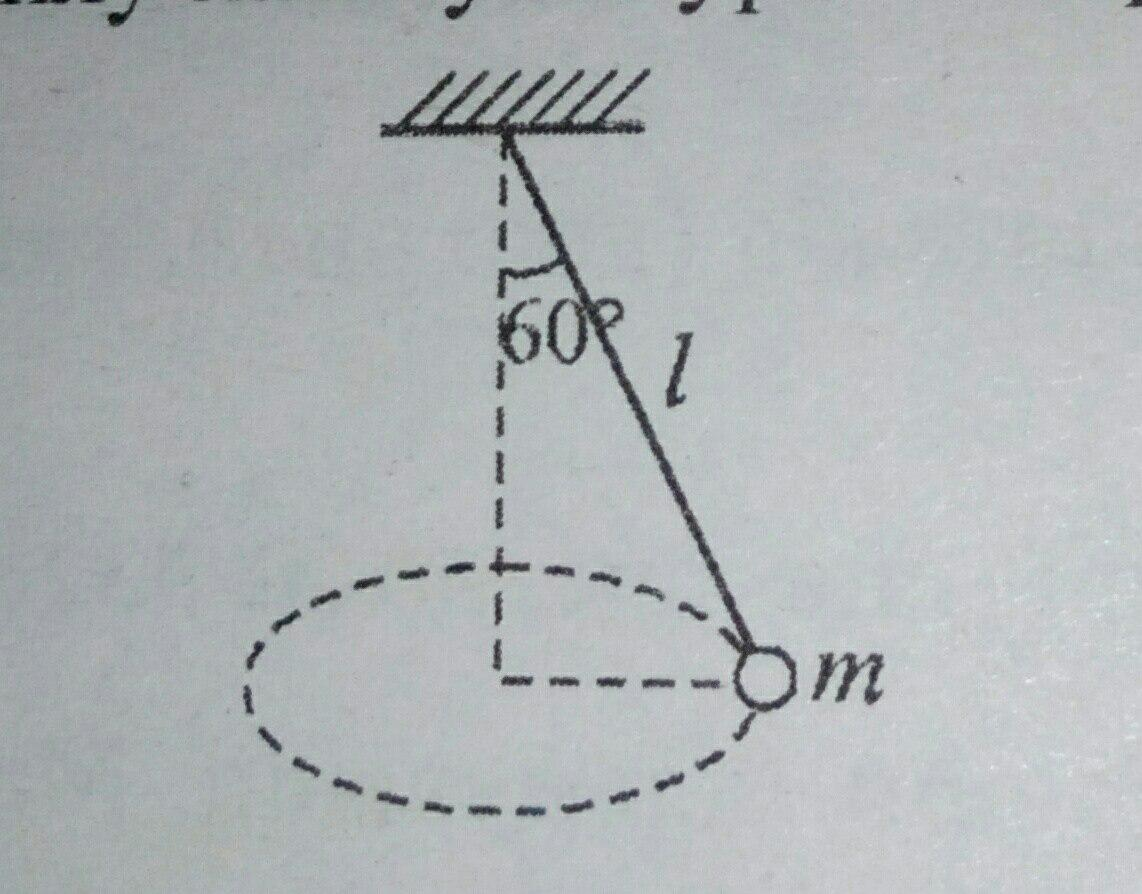
\includegraphics[width=0.5\linewidth]{class5/day5_4}
			\caption{До задачі 5.5}
			\label{fig:day54}
		\end{subfigure}
	\caption{}
	\end{figure}
	
\end{problem}

\begin{problem}{2}
	Чавунне ядро масою $m$ падає у воді з постійною швидкістю $v$. З якою силою $F$ треба тягнути його вверх, щоб воно підіймалось зі швидкістю $2v$? Вважайте, що сила опору води пропорційна швидкості ($\vec{F} = -k\vec{v}$)
\end{problem}

\begin{problem}{3}
	Клин з кутом $90^{\circ}$ при верхній вершині та кутами $\alpha~i~\beta$ при основі розміщений на гладкому столі. По його бокових гранях одночасно поинають ковзати без тертя бруски однакової маси. Чи буде при цьому клин ковзати по столу? (рис. \ref{fig:day502})
	
\end{problem}

\begin{problem}{4}
	З верхньої точки вертикального диску радіуса $R$ прорізаний жолоб. Як залежить від кута $\beta$ час зісковзання $t$ по жолобу? (рис. \ref{fig:day53})
	
\end{problem}

\begin{problem}{5}
	Вантаж, маса якого дорівнює $0.1$ кг, підвішений до шнура завдовжки $1$ м і рухається рівномірно по горизонтальному колу так, що шнур описує конічну поверхню та відхиляється від вертикалі на $60^{\circ}$. Визначити силу натягу шнура та період обертання вантажу. (рис. \ref{fig:day54})
	
\end{problem}

\begin{problem}{6}
	%Goncharenko Olimpiady 2.110%
	
	Яку максимальну силу можно прикласти до нижнього бруска (див. рис. \ref{fig:gon_2110}) щоб верхній брусок утримувався без проковзування на його поіерхні при рівноприскореному русі нижнього по горизонтальній площині? Коефіцієнт тертя між брусками $\mu_1 = 1$ кг, нижнього $m_2 = 2$ кг.
	
	\begin{figure}[h!]
		\centering
		\begin{subfigure}{.4\textwidth}
			\centering
			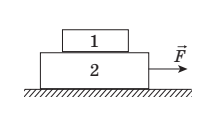
\includegraphics[width=0.5\linewidth]{class5/gon_2110}
			\caption{}
			\label{fig:gon2110}
		\end{subfigure}
		\begin{subfigure}{.4\textwidth}
			\centering
			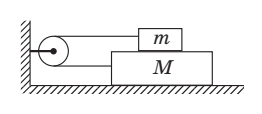
\includegraphics[width=0.5\linewidth]{class5/gon_2113}
			\caption{}
			\label{fig:gon2113}
		\end{subfigure}
		\caption{}
	\end{figure}
\end{problem}

\begin{problem}{6}
	Кінці А та В стержня АВ ковзають по сторонах прямого кута. Як залежить від кута $\alpha$ прискорення середини стержня С, якщо кынець В рухається з постыйною швидкістю $v$ (рис. \ref{fig:day55})
	
	\begin{figure}[h!]
		\centering
		\begin{subfigure}{.4\textwidth}
			\centering
			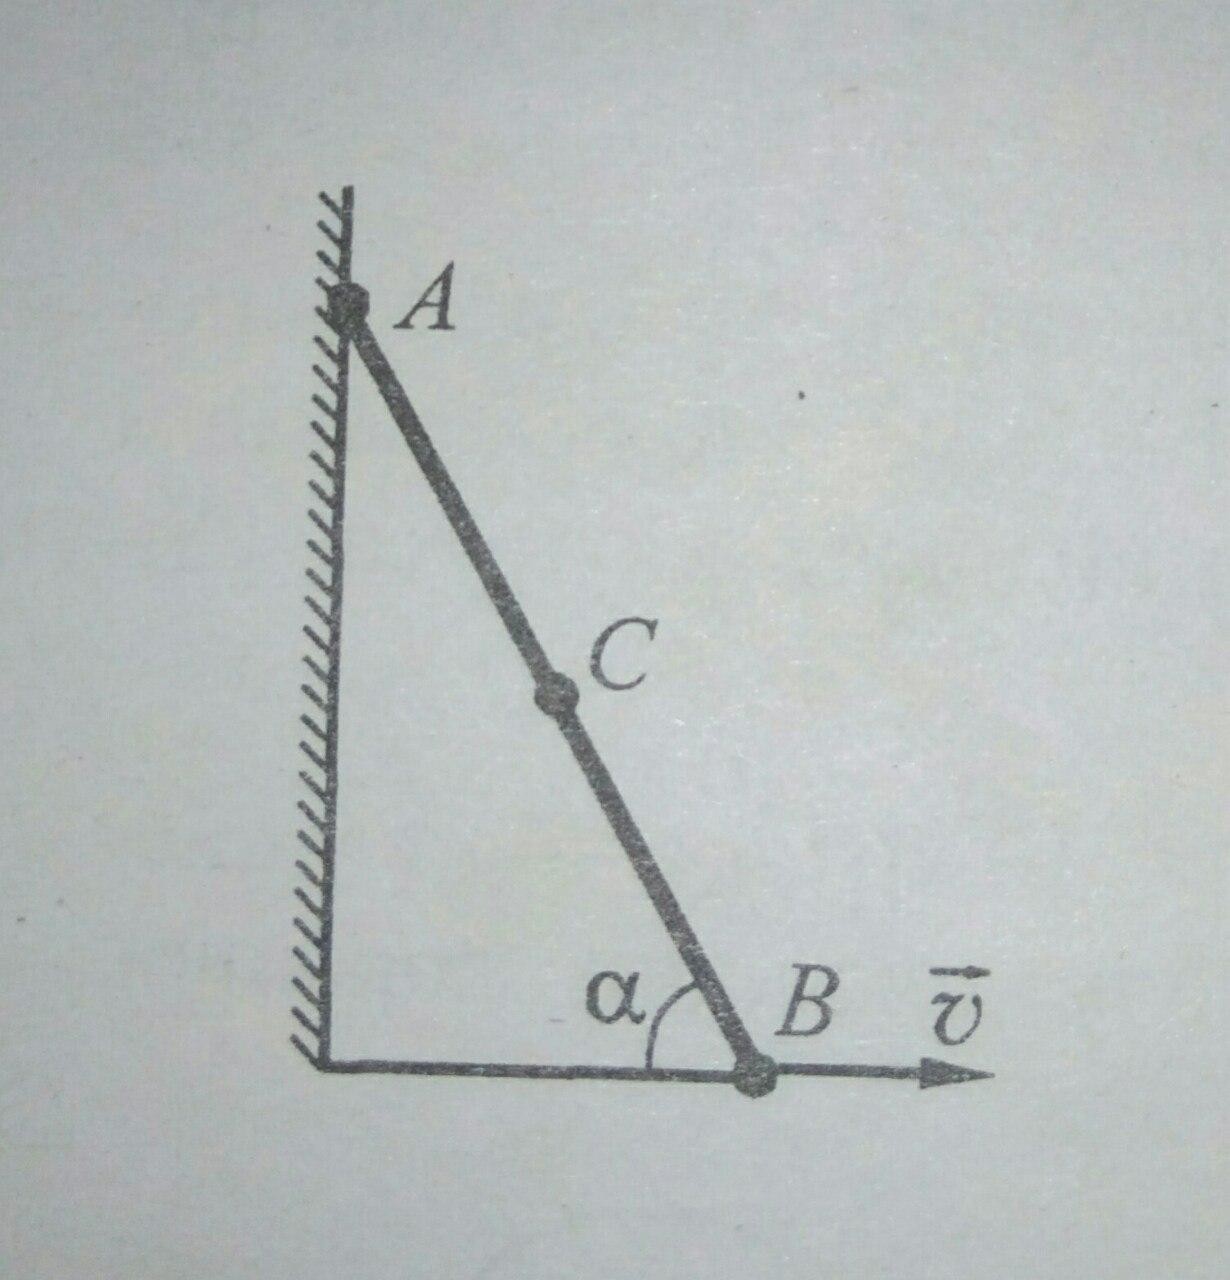
\includegraphics[width=0.5\linewidth]{class5/day5_5}
			\caption{}
			\label{fig:day55}
		\end{subfigure}
		\begin{subfigure}{.4\textwidth}
			\centering
			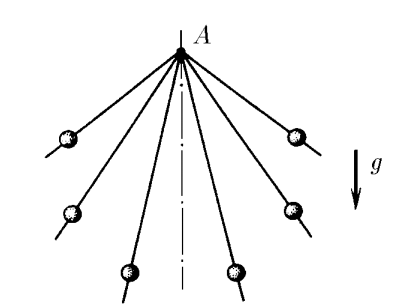
\includegraphics[width=0.5\linewidth]{class3/balls}
			\caption{}
			\label{fig:balls}
		\end{subfigure}
	\caption{}
	\end{figure}
	
\end{problem}

\textbf{Задачі для самостійного розв'язання}

\begin{problem}{3}
	Дві кульки падають в повітрі. Кульки (суцільні) зроблені з одного матеріалу, але діаметр одної вдвічі більше за діаметр другої. Як співвідносяться швидкості встановившогося (рівномірного) руху? Вважати, що сила опору повітря пропорційна площі поперечного перерізу тіл та квадрату швидкості.
\end{problem}

\begin{problem}{4}
	%Kozlov 56%
	Тягач тягне санки з вантажем по обледенілій дорозі зі швидкістю $15~ \dfrac{\text{км}}{\text{год}}$. З якою швидкістю $v_2$ тягач міг би тягнути санки з вантажем при русі дорогою, вкритою деревиною, якщо потужність, яка розвивається мотором одна й та сама? Коефіцієнт тертя при русі обледенілою дорогою $k_1 = 0.01$, а по дорозы. вкритою деревиною -- $k_2 = 0.15$
\end{problem}

\begin{problem}{5}
	%Kozlov 63%
	Тіло, яке кинули вертикально вгору з початковою швидкістю $v_0 = 30~\dfrac{\text{м}}{\text{с}} $, досягає найвищої точки підйому через час $t = 2.5$ c. Маса тіла $40$ г. Знайти середню силу опору повітря $f$, яка діє на тіло піл час руху. 
\end{problem}


\begin{problem}{8}
	З точки А по спицям з різним нахилом одночасно починають зісковзати без тертя маленьки бусинки. На якій кривій будуть знаходитись бусинки в момент часу $t$? (див. рис. \ref{fig:balls})

	(Вказівка: виведіть рівняння кола не відносно центра кола, а відносно точки на колі. Застосуйте знання з векторів)	
\end{problem}

\begin{problem}{9}
	На гладенькому горизонтальному столі лежить брусок  масою $M = 2$ кг, на якому знаходиться другий брусок масою $m = 1$ кг (див.рис. \ref{fig:gon2113}). Обидва бруски з'єднані невагомою нерозтяжною ниткою, перекинутою через невагомий блок. Яку силу $F$ треба прикласти до нижнього бруска, щоб він почав віддалятися від блока з постійним прискоренням $a_1 = \dfrac{1}{2}g$? Коефіцієнт тертя між брусками $\mu = 0.5$/ Тертям між нижнім бруском і столом, а також тертям у блоці знехтувати.
\end{problem}